% Switchyard — DevOps interview preparation guide
% Compile:  pdflatex docs/DEVOPS-INTERVIEW-GUIDE.tex   (run twice for refs)
\documentclass[10pt,a4paper]{article}

\usepackage[margin=16mm,top=14mm,bottom=16mm]{geometry}
\usepackage[T1]{fontenc}
\usepackage{lmodern}
\usepackage{xcolor}
\usepackage{booktabs}
\usepackage{tabularx}
\usepackage{enumitem}
\usepackage{listings}
\usepackage{tikz}
\usepackage{titlesec}
\usepackage[hidelinks]{hyperref}
\usetikzlibrary{positioning,arrows.meta,fit,backgrounds,calc}

\definecolor{ink}{HTML}{15181D}
\definecolor{accent}{HTML}{2B5FD9}
\definecolor{ok}{HTML}{1A7F4B}
\definecolor{warn}{HTML}{9A6400}
\definecolor{bad}{HTML}{B3261E}
\definecolor{soft}{HTML}{F2F4F8}
\definecolor{line}{HTML}{C8CFD9}

\titleformat{\section}{\large\bfseries\color{accent}}{\thesection}{0.6em}{}
\titlespacing*{\section}{0pt}{10pt}{4pt}
\titleformat{\subsection}{\normalsize\bfseries}{\thesubsection}{0.5em}{}
\titlespacing*{\subsection}{0pt}{7pt}{2pt}
\setlist{nosep,leftmargin=1.1em}
\setlength{\parindent}{0pt}
\setlength{\parskip}{3pt}

\lstset{
  basicstyle=\ttfamily\scriptsize,
  backgroundcolor=\color{soft},
  frame=leftline, framerule=1.2pt, rulecolor=\color{line},
  xleftmargin=6pt, framexleftmargin=6pt,
  breaklines=true, columns=fullflexible,
  keywordstyle=\color{accent}, commentstyle=\color{ok}\itshape,
  showstringspaces=false, aboveskip=4pt, belowskip=4pt,
}

% Status marks used throughout.
\newcommand{\done}{\textcolor{ok}{\textbf{[built]}}}
\newcommand{\unver}{\textcolor{warn}{\textbf{[unverified]}}}
\newcommand{\plan}{\textcolor{bad}{\textbf{[planned]}}}

\begin{document}

\begin{center}
  {\LARGE\bfseries Switchyard — DevOps Interview Guide}\\[2pt]
  {\small A multi-tenant LLM gateway, its pipeline, and the numbers I can defend.}\\[2pt]
  {\footnotesize Branch \texttt{devops} · 8 commits · generated 25 Oct 2026 ·
   every figure here is from the repository or a recorded run}
\end{center}

\vspace{-4pt}
\section{What Switchyard is, and the problem}

Switchyard is a \textbf{multi-tenant LLM gateway}: several teams send
OpenAI-format requests to one endpoint, and it decides who is served, in what
order, and what happens when a provider breaks.

\textbf{The problem it exists for.} LLM traffic cannot be scheduled like HTTP
traffic, for two reasons:

\begin{itemize}
\item \textbf{Capacity is not fungible.} A request holds a provider slot for as
  long as it generates, and how long that is depends on output length — which
  the caller does not declare and the model does not promise. Limiting by
  requests-per-second allocates the wrong unit: one tenant sending 4{,}000-token
  completions consumes roughly ten times the resource of one sending 400-token
  completions at the same rate, and is charged the same.
\item \textbf{Failure is not uniform.} A provider that is slow, one returning
  5xx, and one that answered and then went silent mid-stream need three
  different responses. A single timeout treats them identically.
\end{itemize}

Switchyard schedules in \textbf{tokens}, enforces budgets as a \textbf{hard
bound}, and decomposes timeouts into connect / first-token / inter-token /
total so each failure gets its own handling.

\subsection{Tech stack}

\begin{tabularx}{\textwidth}{@{}lX@{}}
\toprule
\textbf{Layer} & \textbf{Choice and why} \\
\midrule
Runtime & Python 3.14, asyncio, uvloop + httptools. IO-bound workload; the
  analysis half of the project (numpy, pyarrow, matplotlib) matters more than
  raw throughput. \\
Web & FastAPI / Starlette, \texttt{httpx} for upstream, \texttt{orjson}. \\
Observability & \texttt{prometheus-client} (own registry), Grafana, structured
  JSON logs with a redaction guard. \\
Frontend & Plain HTML/CSS/ES modules + SVG. No framework, no build step. \\
Packaging & One Docker image, three entrypoints (gateway, synthetic fleet,
  console). Base image pinned by multi-arch digest. \\
CI & GitHub Actions on \texttt{ubuntu-24.04}, every action pinned to a commit
  SHA. \\
Planned infra & One EC2 \texttt{t3.micro}, Docker Compose, SSM Parameter Store,
  GitHub OIDC. Target cost \$0. \\
\bottomrule
\end{tabularx}

\subsection{Five decisions worth defending}

\begin{enumerate}
\item \textbf{Single process, by design.} The scheduler is in-process. Two
  gateways would each claim all upstream capacity and both write the spend
  file, so deploys are \emph{recreate with drain}, never rolling.
\item \textbf{Budgets reserve the ceiling, not the estimate.} A scheduling
  mis-estimate self-corrects at settlement; a budget mis-estimate is money
  already spent. Reserving \texttt{max\_tokens} makes
  \texttt{spent + reserved <= limit} true by construction, and the request's
  \texttt{max\_tokens} is clamped to the headroom that remains.
\item \textbf{Failover is phased.} Before the first token, another provider
  serves the request invisibly. After it, never — splicing a second
  continuation onto a partial answer returns corrupted output under a 200.
  Instead the stream ends with a typed error carrying tokens delivered.
\item \textbf{Liveness and readiness are different endpoints.} Readiness gates
  traffic; liveness gates restarts. They disagree exactly during drain, where
  a restart would destroy the in-flight work the drain protects.
\item \textbf{No framework on the console.} Four static files let the Content
  Security Policy stay \texttt{default-src 'self'} with no
  \texttt{unsafe-inline}, which tests enforce.
\end{enumerate}

\newpage
\section{Architecture}

\begin{center}
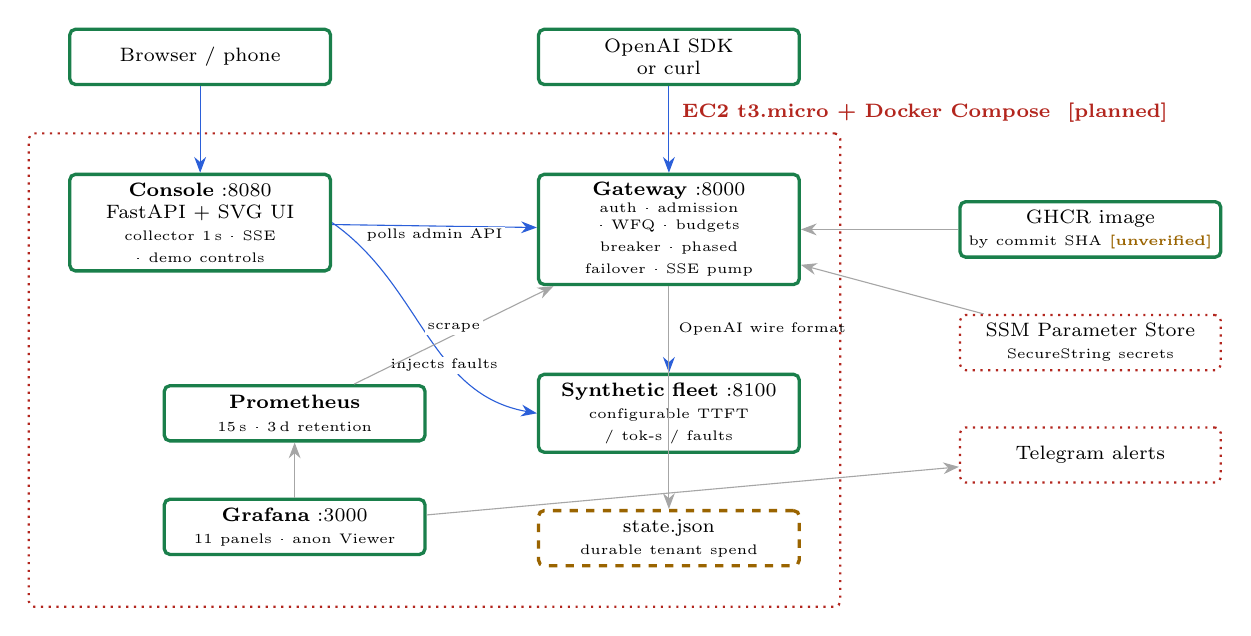
\begin{tikzpicture}[
  font=\scriptsize,
  nodebox/.style={draw=line,fill=white,rounded corners=2pt,minimum height=7mm,
              align=center,inner sep=3pt,text width=31mm},
  isbuilt/.style={nodebox,draw=ok,very thick},
  isunv/.style={nodebox,draw=warn,very thick,dashed},
  planned/.style={nodebox,draw=bad,thick,dotted},
  flow/.style={-{Stealth[length=2mm]},draw=accent,thin},
  faint/.style={-{Stealth[length=2mm]},draw=gray!70,thin},
]
% clients
\node[isbuilt] (phone) {Browser / phone};
\node[isbuilt,right=26mm of phone] (sdk) {OpenAI SDK\\or curl};

% host box contents
\node[isbuilt,below=11mm of phone] (console) {\textbf{Console} :8080\\FastAPI + SVG UI\\
  \tiny collector 1\,s · SSE · demo controls};
\node[isbuilt,below=11mm of sdk] (gw) {\textbf{Gateway} :8000\\
  \tiny auth · admission · WFQ · budgets\\\tiny breaker · phased failover · SSE pump};
\node[isbuilt,below=11mm of gw] (fleet) {\textbf{Synthetic fleet} :8100\\
  \tiny configurable TTFT / tok-s / faults};
\node[isbuilt,left=14mm of fleet] (prom) {\textbf{Prometheus}\\\tiny 15\,s · 3\,d retention};
\node[isbuilt,below=7mm of prom] (graf) {\textbf{Grafana} :3000\\\tiny 11 panels · anon Viewer};
\node[isunv,below=7mm of fleet] (state) {state.json\\\tiny durable tenant spend};

% ec2 frame
\begin{scope}[on background layer]
  \node[planned,fit=(console)(gw)(fleet)(prom)(graf)(state),
        inner sep=5mm,label={[font=\scriptsize\bfseries,text=bad]above right:%
        EC2 t3.micro + Docker Compose \ \plan}] (ec2) {};
\end{scope}

% external
\node[isbuilt,right=20mm of gw] (ghcr) {GHCR image\\\tiny by commit SHA \unver};
\node[planned,below=7mm of ghcr] (ssm) {SSM Parameter Store\\\tiny SecureString secrets};
\node[planned,below=7mm of ssm] (tg) {Telegram alerts};

\draw[flow] (phone) -- (console);
\draw[flow] (sdk) -- (gw);
\draw[flow] (console) -- node[midway,below,font=\tiny,fill=white,inner sep=1pt]{polls admin API} (gw);
\draw[flow] (gw) -- node[midway,right,font=\tiny]{OpenAI wire format} (fleet);
\draw[flow] (console.east) to[out=-35,in=170]
   node[pos=0.6,below,font=\tiny,fill=white,inner sep=1pt]{injects faults} (fleet.west);
\draw[faint] (prom) -- node[midway,above,font=\tiny,fill=white,inner sep=1pt]{scrape} (gw);
\draw[faint] (graf) -- (prom);
\draw[faint] (gw) -- (state);
\draw[faint] (ghcr) -- (gw);
\draw[faint] (ssm) -- (gw);
\draw[faint] (graf) -- (tg);
\end{tikzpicture}
\end{center}

\vspace{-2pt}
{\footnotesize \done\ implemented and tested \quad
\unver\ implemented, not yet verified end to end \quad
\plan\ not built yet}

\subsection{What each component does}

\begin{tabularx}{\textwidth}{@{}p{30mm}p{34mm}X@{}}
\toprule
\textbf{Component} & \textbf{Path} & \textbf{Implementation} \\
\midrule
Scheduler & \texttt{core/scheduler.py} &
  Weighted fair queueing on per-tenant virtual clocks, in tokens. Floors,
  ceilings, work-conserving shared pool. Capacity is an async context
  manager, so a leaked lease is impossible by construction. \\
Queue policies & \texttt{core/queueing.py} &
  \texttt{settle()} corrects the virtual clock against actual consumption;
  \texttt{FifoQueue} is the baseline arm of the experiment. \\
Budgets & \texttt{core/budget.py} &
  Three distinct quantities: estimate (p50), reservation
  (\texttt{max\_tokens}), actual. Clamps rather than overspends. \\
Durability & \texttt{core/persistence.py} &
  Spend written whole, fsynced, moved with \texttt{os.replace}. Batched: a
  crash under-charges by at most one flush interval, never over-charges. \\
Reliability & \texttt{core/health.py}, \texttt{routing.py} &
  Rolling-window breaker, \texttt{min\_samples}, jittered doubling cooldown,
  bounded half-open probes; phased failover. \\
HTTP surface & \texttt{gateway/app.py} &
  \texttt{/v1/chat/completions}, \texttt{/livez}, \texttt{/readyz},
  \texttt{/metrics}, \texttt{/v1/scheduler/stats}, \texttt{/v1/providers},
  \texttt{/v1/admin/drain}. \\
Console backend & \texttt{console/} &
  1\,s collector over four sources; counter deltas $\rightarrow$ rates; p95
  from histogram bucket deltas; HMAC cookie; SSE. \\
Console UI & \texttt{console/static/} &
  Four files, no build step. SVG map, hash routes, one \texttt{EventSource}. \\
Instruments & \texttt{synthetic/}, \texttt{bench/} &
  Deterministic fault-injecting provider fleet; open-loop load generator. \\
\bottomrule
\end{tabularx}

\subsection{Request path, in order}

\texttt{auth (SHA-256 + pepper, constant-time)} $\rightarrow$
\texttt{validate} $\rightarrow$ \texttt{estimate p50} $\rightarrow$
\texttt{admission + WFQ (bounded queue, deadline)} $\rightarrow$
\texttt{budget reserve + clamp} $\rightarrow$
\texttt{route bind at dispatch} $\rightarrow$
\texttt{provider stream} $\rightarrow$
\texttt{settle (fairness clock + budget)}.

The route is bound at \emph{dispatch}, not at admission: provider health
changes while a request sits in the queue, so a route chosen four seconds ago
may point at a circuit that has since opened.

\newpage
\section{CI/CD pipeline}

\begin{center}
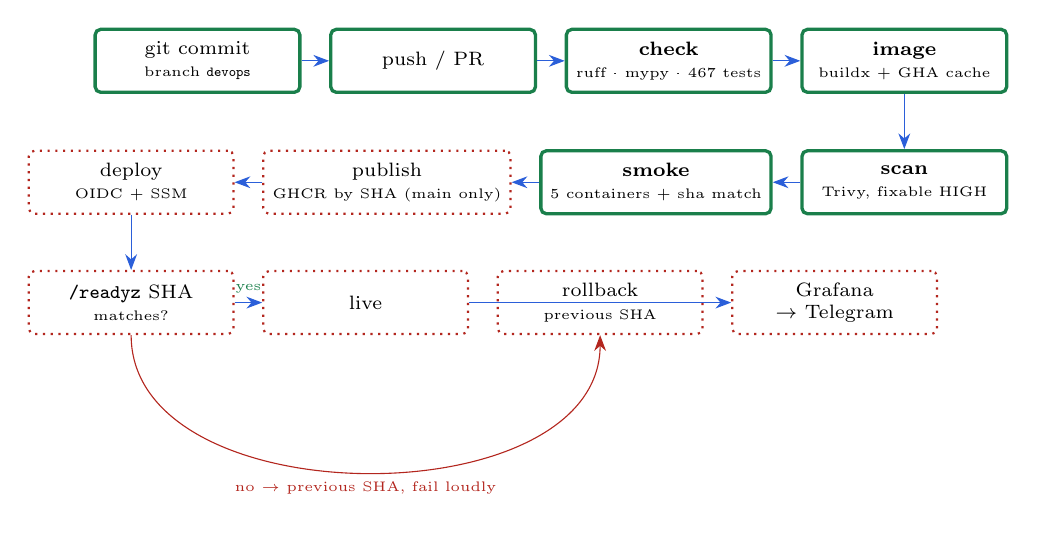
\begin{tikzpicture}[
  font=\scriptsize, node distance=3.5mm,
  stage/.style={draw=ok,very thick,fill=white,rounded corners=2pt,
               minimum width=26mm,minimum height=8mm,align=center},
  later/.style={stage,draw=bad,thick,dotted},
  arr/.style={-{Stealth[length=2mm]},draw=accent},
]
\node[stage] (commit) {git commit\\\tiny branch \texttt{devops}};
\node[stage,right=of commit] (pr) {push / PR};
\node[stage,right=of pr] (check) {\textbf{check}\\\tiny ruff · mypy · 467 tests};
\node[stage,right=of check] (img) {\textbf{image}\\\tiny buildx + GHA cache};
\node[stage,below=7mm of img] (scan) {\textbf{scan}\\\tiny Trivy, fixable HIGH};
\node[stage,left=of scan] (smoke) {\textbf{smoke}\\\tiny 5 containers + sha match};
\node[later,left=of smoke] (pub) {publish\\\tiny GHCR by SHA (main only)};
\node[later,left=of pub] (deploy) {deploy\\\tiny OIDC + SSM};
\node[later,below=7mm of deploy] (verify) {\texttt{/readyz} SHA\\\tiny matches?};
\node[later,right=of verify] (live) {live};
\node[later,right=of live] (rollback) {rollback\\\tiny previous SHA};
\node[later,right=of rollback] (alert) {Grafana\\$\rightarrow$ Telegram};

\draw[arr] (commit) -- (pr);
\draw[arr] (pr) -- (check);
\draw[arr] (check) -- (img);
\draw[arr] (img) -- (scan);
\draw[arr] (scan) -- (smoke);
\draw[arr] (smoke) -- (pub);
\draw[arr] (pub) -- (deploy);
\draw[arr] (deploy) -- (verify);
\draw[arr] (verify) -- node[midway,above,font=\tiny,text=ok]{yes} (live);
\draw[arr,draw=bad] (verify.south) to[out=-90,in=-90]
   node[midway,below,font=\tiny,text=bad]{no $\rightarrow$ previous SHA, fail loudly} (rollback.south);
\draw[arr] (live) -- (alert);
\end{tikzpicture}
\end{center}

{\footnotesize Solid green = running today on every push. Dotted red = written
or specified but \textbf{not yet executed}. The honest summary: \textbf{the
test stage is real and green; everything from image publication onward is
designed, and M5--M8 build it.}}

\subsection{The bug that kept CI red for two months}

\begin{lstlisting}[language=bash]
# CI ran:          pytest -q          -> ModuleNotFoundError: No module named 'tests'
# The Makefile ran: python -m pytest  -> 465 passed
\end{lstlisting}

\texttt{python -m X} prepends the working directory to \texttt{sys.path}; the
console script does not. Eleven test call sites do
\texttt{from tests.conftest import ...}, and the module-scope one aborted
collection — \textbf{exit code 2 after four seconds, so zero tests ran since
28 August}, while \texttt{ruff} and \texttt{mypy} stayed green because neither
imports the package. The fix declares the requirement instead of relying on
how pytest is launched:

\begin{lstlisting}
[tool.pytest.ini_options]
pythonpath = ["."]          # both invocations now behave identically
\end{lstlisting}

\subsection{Pipeline configuration, with the lines that matter}

\begin{lstlisting}
jobs:
  check:
    runs-on: ubuntu-24.04                       # pinned: 'latest' was migrating to Ubuntu 26
    steps:
      - uses: actions/checkout@3d3c42e5aac5...  # v7.0.1 -- SHA, not tag: a tag can be repointed
      - name: Environment
        run: python -VV && uname -a && pip freeze   # so the next red run is diagnosable
      - name: Collect tests
        run: pytest --collect-only -q           # "could not load" != "a test failed"
      - run: pytest -q
\end{lstlisting}

\begin{lstlisting}
# deploy/compose.prod.yml -- the two lines that are easy to get wrong
stop_grace_period: 40s        # drain is 30s; Docker SIGKILLs at 10s by default,
                              # so every graceful shutdown was cut to a third
healthcheck:                  # readiness, not liveness: depends_on asks
  test: [... '/readyz']       # "can this take traffic", and draining cannot
\end{lstlisting}

\textbf{Secrets flow} (designed, not yet run): SSM SecureString $\rightarrow$
\texttt{deploy.sh} writes \texttt{/etc/switchyard/*.env} (one per service,
mode 600) $\rightarrow$ one env file per service, so the gateway never sees the
console password and Grafana never sees the key pepper. GitHub authenticates
to AWS by OIDC, so no long-lived key is stored.

\section{Numbers I can defend}

\subsection{Measured — from recorded runs}

\begin{tabularx}{\textwidth}{@{}p{52mm}p{30mm}p{30mm}X@{}}
\toprule
\textbf{Result} & \textbf{Baseline} & \textbf{Switchyard} & \textbf{Source} \\
\midrule
Queue wait p95, protected tenant under a flood & 19{,}980\,ms (FIFO) &
  \textbf{273\,ms} (token-fair) & \texttt{results/fairness\_summary.json} \\
Latency p95, same tenant & 24{,}449\,ms & \textbf{5{,}522\,ms} & same \\
Token share, same tenant & 9.2\,\% & 13.5\,\% & same \\
Requests served during a total provider outage & 16/120 (\textbf{13\,\%}) &
  48/48 (\textbf{100\,\%}) & \texttt{results/outage\_summary.json} \\
Transparent failovers in that window & 0 & 26 & same \\
Requests that skipped the dead provider & 176 & 34 & same \\
Gateway TTFT p50 (synthetic fleet, 2--40\,rps) & \multicolumn{2}{l}{218--240\,ms, flat across the sweep} &
  \texttt{results/baseline\_rate*.parquet} \\
End-to-end latency p99 at 40\,rps & \multicolumn{2}{l}{3{,}403\,ms} & same \\
Console, live: flooding tenant & \multicolumn{2}{l}{106 queued, 12{,}200\,ms wait} &
  browser run, 25 Oct \\
Console, live: protected tenant & \multicolumn{2}{l}{0 queued, \textbf{1\,ms} wait} & same \\
\bottomrule
\end{tabularx}

\subsection{Verified engineering facts}

\begin{tabularx}{\textwidth}{@{}p{58mm}X@{}}
\toprule
\textbf{Fact} & \textbf{Evidence} \\
\midrule
\textbf{472 automated tests} (465 fast + 7 slow), ruff and mypy clean &
  \texttt{make check}, \texttt{make test-all} exit 0 \\
mypy \texttt{disallow\_untyped\_defs} on \texttt{core} and \texttt{adapters} &
  \texttt{pyproject.toml} override \\
CI green on 4 consecutive runs & runs \texttt{40191532932}, \texttt{40199010161},
  \texttt{40206654225}, \texttt{40209249206} \\
$\approx$10{,}000 lines of Python across 51 modules; 5{,}963 lines of tests
  across 24 files; 1{,}431 lines of frontend & \texttt{wc -l} \\
Spend survives restart & live test: 150 tokens $\rightarrow$ restart
  (\texttt{restored\_tokens=150}) $\rightarrow$ 301 \\
Provider-outage demo passes end to end with no API key &
  \texttt{test\_console\_api.py}, 37\,s \\
\bottomrule
\end{tabularx}

\subsection{Configured limits — not measurements}

\begin{tabularx}{\textwidth}{@{}p{46mm}p{30mm}X@{}}
\toprule
\textbf{Setting} & \textbf{Value} & \textbf{Reason} \\
\midrule
Gateway capacity & 24 dev / \textbf{12 prod} & What a \texttt{t3.micro}
  running five containers can serve. \\
Tenant floors (prod) & 4 / 3 / 1 of 12 & Little's law against offered rate;
  4 slots stay shared. \\
Queue depth (prod) & 40 / 64 / 32 & 256 absorbed the demo flood by queueing
  and hid admission control. \\
Budgets & 2\,M / 500\,k / 50\,k tokens & Lifetime totals; no refill window yet. \\
Timeouts & 2 / 8 / 10 / 300\,s & connect / first-token / inter-token / total. \\
Breaker & 50\,\% of $\geq$10 samples, 5\,s jittered doubling, 2 probes & \\
Drain / stop grace & 30\,s / 40\,s & Docker's default 10\,s SIGKILL was cutting it. \\
Scrape interval & 1\,s dev / 15\,s prod & 1\,s resolves a recovery timeline;
  15\,s is what the box should carry. \\
Console caps & 30\,rps, 120 streams, 120\,s & Enforced in
  \texttt{Profile.validate()} and tested. \\
\bottomrule
\end{tabularx}

\subsection{Not verified — say so plainly}

\begin{itemize}
\item \textbf{\texttt{publish} has never run.} It is gated on a push to
  \texttt{main} and this work is on a branch, so no image exists in GHCR
  yet. \unver
\item \textbf{\texttt{make prod-local} has not completed on this laptop} --
  the pinned Prometheus and Grafana images are still pulling -- so there are
  no \texttt{docker stats} figures and no decision on memory limits. The same
  compose files do run green in CI. \unver
\item \textbf{Nothing is deployed to AWS.} No Terraform, no instance, no
  image in GHCR, no alerts. \plan
\item No HA, no TLS, budgets are lifetime totals, and the console session
  cookie cannot be \texttt{Secure} on plain HTTP.
\end{itemize}

\section{Interview preparation}

\subsection{Sixty-second introduction}

\textit{``Switchyard is a multi-tenant LLM gateway. The problem is that LLM
requests aren't fungible — a request holds a provider slot for as long as it
generates, and nobody knows how long that is until it's done. So rate-limiting
by requests-per-second allocates the wrong unit: one tenant sending long
completions can starve everyone else while looking perfectly well-behaved on a
request counter.}

\textit{It schedules in tokens instead, with reserved capacity floors per
tenant, hard token budgets, and circuit breaking with failover. The part I'm
proudest of is that it ships with the harness that breaks it: a synthetic
provider fleet and a web console where you press a button, one tenant floods
at 25 requests a second, and you watch the protected tenant hold a 1-millisecond
queue wait while the flooder backs up to twelve seconds. The verdicts are
scored from the same measurements the map draws, so the demo can fail — and it
has, in front of me, which is how I found four bugs.''}

\subsection{Three-minute technical version}

\begin{enumerate}
\item \textbf{The scheduling problem} (30\,s) — tokens not requests; the 10×
  example; floors sized by Little's law.
\item \textbf{Reliability} (45\,s) — four timeouts not one; \texttt{min\_samples}
  so one unlucky request can't trip the breaker; failover phased on whether a
  token already reached the client, because splicing two answers is corruption
  under a 200.
\item \textbf{Proving it} (45\,s) — open-loop load generation avoids
  coordinated omission; FIFO vs token-fair as two arms of one experiment;
  19{,}980\,ms $\rightarrow$ 273\,ms queue wait, 13\,\% $\rightarrow$ 100\,\%
  outage survival.
\item \textbf{The pipeline} (45\,s) — CI had been red for two months; the cause
  was \texttt{pytest} versus \texttt{python -m pytest}, so \emph{no test had
  run} since August while the badge said only that the job failed. Fixed the
  cause, pinned the runner and every action SHA, added an environment dump and
  a separate collection step.
\item \textbf{What's left} (15\,s) — image build unverified, AWS not deployed,
  and I will say so.
\end{enumerate}

\subsection{Questions and short answers}

\begin{tabularx}{\textwidth}{@{}p{54mm}X@{}}
\toprule
\textbf{Question} & \textbf{Answer} \\
\midrule
Liveness vs readiness? &
  Readiness gates traffic, liveness gates restarts. They differ during drain:
  readiness must fail so the load balancer stops sending, liveness must hold
  or the orchestrator kills the in-flight work the drain exists to finish.
  \texttt{/livez} reads no scheduler state on purpose. \\
Why recreate-with-drain, not rolling? &
  The scheduler is in-process and there is one spend file. Two gateways would
  each claim all upstream capacity and both write it. The cost is a few
  seconds of 503 during drain, which is a deliberate trade. \\
How do you know a deploy worked? &
  \texttt{/readyz} reports the \texttt{git\_sha} baked in at build time, and
  the smoke test compares it to the SHA that was shipped — in the same request
  that proves the gateway is up. A rollback is confirmed the same way. \\
Why pin action SHAs? &
  A tag can be repointed at new code; a commit SHA cannot. The version stays
  in a comment so the pin is still readable. Same argument for the base image
  digest. \\
How do secrets reach the box? &
  SSM SecureString $\rightarrow$ root-only env files, one per service, so the
  blast radius of any one file is one container. GitHub assumes an AWS role by
  OIDC, so there is no stored access key. Nothing secret is in git; key
  \emph{digests} are, and they are useless without the pepper. \\
Your security scan failed. What did you do? &
  Four fixable HIGH advisories, all in tooling rather than my dependencies:
  setuptools, and urllib3 and msgpack vendored inside pip. A service that
  runs \texttt{uvicorn} never installs anything, so I removed pip,
  setuptools and wheel from the runtime image -- that deletes the vulnerable
  code rather than upgrading it. The gate ignores unfixed CVEs, because a
  gate that cannot be satisfied is one people route around. \\
Why is breaker-open a warning, not critical? &
  Because failover already protected the user. The page-worthy signal is
  client-visible error rate, which is what actually reached someone. \\
What broke, and what did you learn? &
  CI assumed a developer's machine in three places: how pytest was launched,
  that a \texttt{.venv} exists, and that a benchmark window always has data.
  Separately, running the console in a browser found three bugs no API test
  could — all of them between a correct client and a correct server. \\
What would you do with a budget? &
  HTTPS at a load balancer, spend moved out of the process so a new version
  starts from current spend, and only then multiple replicas — admission state
  has to be shared first, behind the existing \texttt{Scheduler} seam. \\
\bottomrule
\end{tabularx}

\subsection{Resume bullets — verified only}

\begin{enumerate}[leftmargin=1.4em]
\item Built a multi-tenant LLM gateway with token-denominated weighted fair
  queueing and reserved capacity floors; under a 25\,rps single-tenant flood a
  protected tenant's p95 queue wait fell from \textbf{19{,}980\,ms to 273\,ms}
  (\textbf{73×}) and p95 latency from \textbf{24{,}449\,ms to 5{,}522\,ms}
  against a FIFO baseline, measured with an open-loop, coordinated-omission-free
  load generator.
\item Designed phased failover and a rolling-window circuit breaker that
  carried \textbf{100\,\% of requests (48/48)} through a total provider outage
  versus \textbf{13\,\% (16/120)} without it, with \textbf{26} failovers
  transparent to clients and no partial response ever spliced.
\item Diagnosed and fixed a CI pipeline that had been red for \textbf{two
  months}: \texttt{pytest} versus \texttt{python -m pytest} differ in
  \texttt{sys.path}, so collection aborted and \textbf{zero of 467 tests had
  executed} while linting stayed green. Restored the suite, pinned the runner
  and all action SHAs off deprecated Node 20, and added environment capture.
\item Shipped a zero-dependency web console (four static files, strict CSP
  enforced by tests) that renders live scheduling state from Prometheus
  counter deltas and scores guided failure demos against measured thresholds —
  verified end to end against a synthetic provider fleet with \textbf{no API
  key and no cloud spend}.
\end{enumerate}

\vspace{4pt}
{\footnotesize\itshape Keep this file honest. When the image builds, the stack
runs or AWS is deployed, move those lines out of ``not verified'' — and not
before.}

\end{document}
